\chapter{The functions of the probability theory and statistics}

\section{ Functions of the discrete random quantity}
To define a discrete random quantity, 
enter the matrix, in which the first line~--- values, and the second~--- the corresponding probabilities
(numbers that are in the range from 0 to 1). For example: DRQ = ([1,2,3,4,5],[0.4,0.1,0.1,0.2,0.2]).

There are the following functions for working with discrete random variable:

\comm{mathExpectation}{(DRQ)} calculates the expectation of a discrete random variable $DRQ$. 

\comm{dispersion}{(DRQ)} calculates the variance of a discrete random variable $DRQ$. 

\comm{meanSquareDeviation}{(DRQ)} calculates the standard deviation of a discrete random variable $DRQ$. 

\comm{addQU}{(DRQ1, DRQ2)} adds the two discrete random variables $DRQ1$ and $DRQ2$. 

\comm{multiplyQU}{(DRQ1, DRQ2)} multiplies two discrete random variables $DRQ1$ and $DRQ2$. 

\comm{covariance}{(DRQ1, DRQ2)} calculates the covariance coefficient of two discrete random variables $DRQ1$ and $DRQ2$. 

\comm{correlation}{(DRQ1, DRQ2)} calculates the correlation coefficient of two discrete random variables $DRQ1$ and $DRQ2$. 

\comm{plotPolygonDistribution}{(DRQ, V)} building polygon distributions of discrete random variable $DRQ$. 

\comm{plotDistributionFunction}{(DRQ, V)} constructing the distribution function of a discrete random variable $DRQ$,  
 where $V$~--- is the matrix of one row, 4 elements that define the boundaries Graphics: $[x1, x2, y1, y2]$. 

\comm{simplifyQU}{(DRQ)}  simplify a discrete random variable $DRQ$. 

%begindelete
\underline{Examples:}
%enddelete

\vspace*{-2mm}
\begin{verbatim}
SPACE=R64[x];
M=[[1, 2], [0. 2, 0. 8]];
g=\mathExpectation(M); 
g1=\dispersion(M); 
g2=\meanSquareDeviation(M);  
\print(g, g1, g2);
\end{verbatim}
%begindelete

\ex{$SPACE=R64[x];$\\ 
\hspace*{4mm} $M=\left(\begin{array}{cc}1& 2\\ 0. 2& 0. 8 \end{array}\right);$\\
\hspace*{4mm} $g=mathExpectation(M);$\\ 
\hspace*{4mm} $g1=dispersion(M);$\\ 
\hspace*{4mm} $g2=meanSquareDeviation(M);$\\  
\hspace*{4mm} $print(g, g1, g2);$}
{$g = 1. 8; $\\
\hspace*{4mm} $g1 = 0. 16; $\\
\hspace*{4mm} $g2 = 0. 39;$} 

%enddelete
\begin{verbatim}
SPACE=R64[x]; 
M=[[7, 5, 3, 5, 1], [0. 2, 0. 1, 0. 3, 0. 1, 0. 3]];
g=\simplifyQU(M); 
\print(g);
\end{verbatim}
%begindelete

\ex{$SPACE=R64[x];$\\ 
\hspace*{4mm} $M=\left(\begin{array}{ccccc}   7& 5& 3& 5& 1\\ 0. 2& 0. 1& 0. 3& 0. 1& 0. 3 \end{array}\right);$\\
\hspace*{4mm} $g=simplifyQU(M);$\\ 
\hspace*{4mm} $print(g);$
}
{$g =\left(\begin{array}{cccc}1 &3 &5 &7 \\ 0. 3 &0. 3 &0. 2 &0. 2 \end{array}\right);$}

%enddelete
\begin{verbatim}
SPACE=R64[x]; 
M1=[[0, 1], [0. 33333, 0. 66666]]; 
M2=[[1, 2], [0. 25, 0. 75]];
g=\addQU(M1, M2); 
g1= \multiplyQU(M1, M2);  
\print(g, g1);
\end{verbatim}
%begindelete

\ex{$SPACE=R64[x];$\\ 
\hspace*{4mm} $M1=\left(\begin{array}{cc} 0& 1\\ 0. 33333& 0. 66666  \end{array}\right); $\\
\hspace*{4mm} $M2=\left(\begin{array}{cc} 1& 2\\ 0. 25& 0. 75 \end{array}\right);$\\
\hspace*{4mm} $g=addQU(M1, M2); $\\
\hspace*{4mm} $g1= multiplyQU(M1, M2); $\\ 
\hspace*{4mm} $print(g, g1);$}
{$g =\left(\begin{array}{ccc}1 & 2 & 3\\ 0. 08 &0. 41 &0. 49 \end{array}\right) ; $\\
\hspace*{4mm} $g1 =\left(\begin{array}{ccc}0 & 1 & 2\\ 0. 33 &0. 16 &0. 49 \end{array}\right);$} 

%enddelete
\begin{verbatim}
SPACE=R64[x];
M=[[-7, -2, 0, 3, 5, 7, 9], 
  [0.3, 0.05, 0.2, 0.1, 0.1, 0.2, 0.05]];
V=[-10, 10, 0, 1];
\plotPolygonDistribution(M, V);
\end{verbatim}
%begindelete

 
\ex{$SPACE=R64[x];$\\ 
\hspace*{4mm} $M=\left(\begin{array}{ccccccc} -7& -2& 0& 3& 5& 7& 9\\ 0. 3& 0. 05& 0. 2& 0. 1& 0. 1& 0. 2& 0. 05 \end{array}\right);$\\
\hspace*{4mm} $V=[-10, 10, 0, 1];$\\
\hspace*{4mm} $plotPolygonDistribution(M, V);$}{Pic. \ref{8_1}.}
                       
\begin{figure}[!ht]
 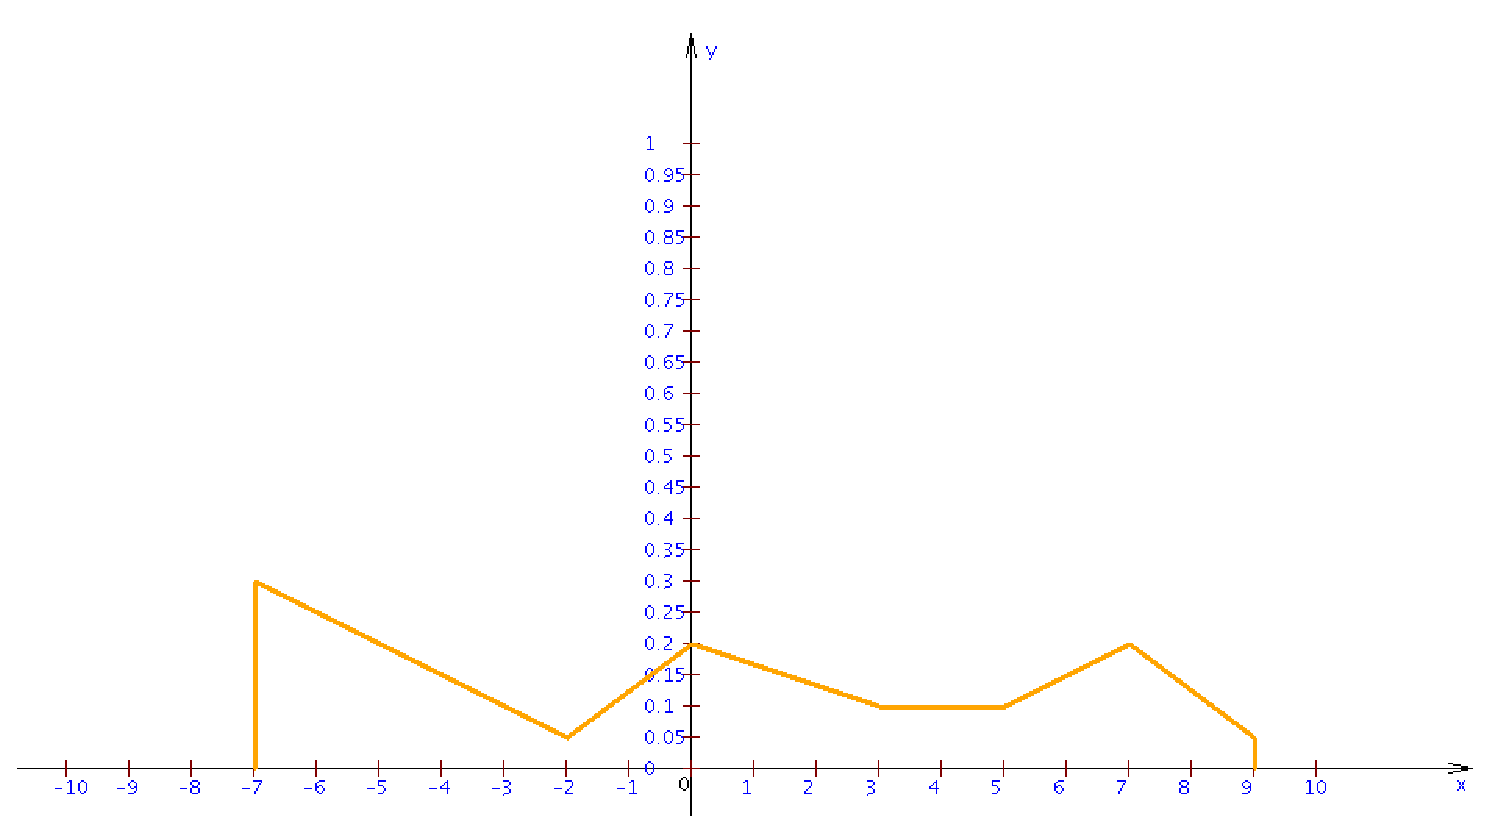
\includegraphics[width=300.57pt, height=192.835pt]{pictures/8_1}
\caption{Polygon of distributions of discrete random variable from the example.
}
\label{8_1}
\end{figure}
%enddelete

\section{Function for sampling}

Function for sampling:

W-matrix of a single line. For example,  $[1, 7, 10, 15]$. 

\comm{sampleMean}{(S)} calculates the sample mean of the sample $S$. 

\comm{sampleDispersion}{(S)} calculates the sample variance of the sample $S$. 

\comm{covarianceCoefficient}{(S1, S2)} calculates the coefficient of covariance for 2 sampling $S1$ and $S2$. 

\comm{correlationCoefficient}{(S1, S2)} calculates the correlation coefficient for 2 sampling $S1$ and $S2$. 

%begindelete
\underline{Example}
%enddelete

\vspace*{-2mm}
\begin{verbatim}
SPACE=R[x, y];
S1=[0, 1]; 
S2=[1, 2];
g=\sampleMean(S1); 
g1=\sampleDispersion(S1); 
g2=\covarianceCoefficient(S1, S2); 
g3=\correlationCoefficient(S1, S2); 
\print(g, g1, g2, g3);
\end{verbatim} 
%begindelete

\ex{$SPACE=R[x, y];$\\
\hspace*{4mm} $S1=[0, 1];$\\ 
\hspace*{4mm} $S2=[1, 2];$\\
\hspace*{4mm} $g=sampleMean(S1); $\\
\hspace*{4mm} $g1=sampleDispersion(S1); $\\
\hspace*{4mm} $g2=covarianceCoefficient(S1, S2); $\\
\hspace*{4mm} $g3=correlationCoefficient(S1, S2);$\\ 
\hspace*{4mm} $print(g, g1, g2, g3);$}
{$g = 0. 5; $\\
\hspace*{4mm} $g1 = 0. 25; $\\
\hspace*{4mm} $g2 = 0. 25; $\\
\hspace*{4mm} $g3 = 1. 00$.} 

%enddelete
 